\chapter{Experiments and Discussions}
For the assessment of the system we performed the measurements listed below
\footnote{
  Unfortunately one of our input channels is not functioning (corresponding to the
  D string), due to a hardware problems (not identified at the timing of writing this document),
  hence it will be ignored. B string signal has DC noise,
  due to resistor imprecisions (not fixed at the time of these experiments),
  which limits the signal peak to peak value, and so it will have poor performance.
}.
Results and discussions are presented in the following sections.

\begin{itemize}
  \item Single Note Accuracy
  \item Chord Accurracy (E and Am)
  \item Chromatic Scale Error
  \item Pluck Counting
\end{itemize}


\section{Single Note Accuracy}
This test is done by hitting a single note in a single string and checking if the correct
frequency is detected. Notes were chosen in order to consider a broad frequency band,
as presented in \autoref{single-note-expected-result}. The amount of detected notes is
not considered in this experiment. \autoref{single-note-result} and \autoref{single-note-accuracy}
present the results. MacLeod presents lower errors.

\begin{table}[htb]
  \begin{center}
    \ABNTEXreducedfont
    \caption[Single Note Expected Result]{Single Note Expected Result}
    \label{single-note-expected-result}
    \begin{tabular}{c | c | c}
      \hline
      String & Frequency(Hz) & Note (name and number)\\
      \hline \hline
      E (6) & 493.9 & B4 (71) \\ \hline
      A (5) & 370 & Gb4 (66) \\ \hline
      G (3) & 293.7 & D4 (62) \\ \hline
      B (2) & 164.8 & E3 (52) \\ \hline
      e (1) & 123.5 & B2 (47) \\ \hline
    \end{tabular}
    \legend{Source: authors}
  \end{center}
\end{table}

\begin{table}[htb]
  \begin{center}
    \ABNTEXreducedfont
    \caption[Single Note Result]{Single Note Result}
    \label{single-note-result}
    \begin{tabular}{c | c | c | c | c}
      \hline
      String & MacLeod Mean (Hz) & MacLeod Standard Deviation & YIN Mean (Hz) & YIN Standard Deviation\\
      \hline \hline
      E (6) & 495.27 & 0.04 & 489.81 & 0.012 \\ \hline
      A (5) & 379.00 & 0.13 & 368.09 & 1.27 \\ \hline
      G (3) & 298.28 & 1.59 & 301.43 & 0.60 \\ \hline
      B (2) & 167.00 & 0.04 & 164.01 & 0.08 \\ \hline
      e (1) & 124.47 & 0.16 & 121.13 & 0 \\ \hline
    \end{tabular}
    \legend{Source: authors}
  \end{center}
\end{table}


\begin{figure}[!htpb]
  \centering
  \caption{Strings Single Note Accuracy}
  \label{single-note-accuracy}
  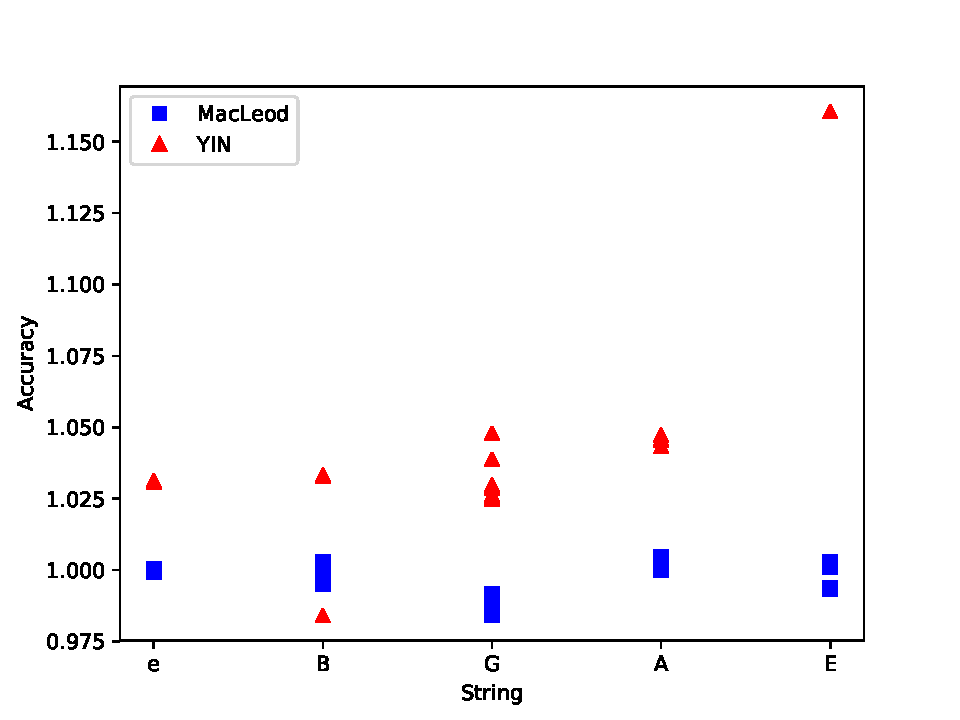
\includegraphics[scale=0.85]{images/measurements/single-note-acc-2}
  \legend{Source: Authors}
\end{figure}

\section{Chord Accuracy (E and Am)}
This experiment aims to assess the performance of the system when simultaneous notes at multiple string are played.
The adopted chords are the E major (E) and A minor (Am). The E chord has it's lower note on
the twelfth fret, to cut off very low frequencies. The Am chord has it's lower note
on the fifth fret, and so lower frequencies.
The error rate and standard deviation were calculated for both cases. The error rate is given by
\autoref{chord-accuracy-equation}. The result can be seen at \autoref{e-chord-error} and \autoref{am-chord-error}, where the
error is given in percentage and the standard deviation in absolute values.
YIN presents lower error, except at low frequencies where it present large error rates.

\begin{equation}
  \label{chord-accuracy-equation}
  Accuracy = \frac{Mean - Expected\ Value}{Expected\ Value} = \frac{\sum x}{Length * Expected\ Value} -1
\end{equation}

\begin{figure}[!htpb]
  \centering
  \caption{Am chord error}
  \label{am-chord-error}
  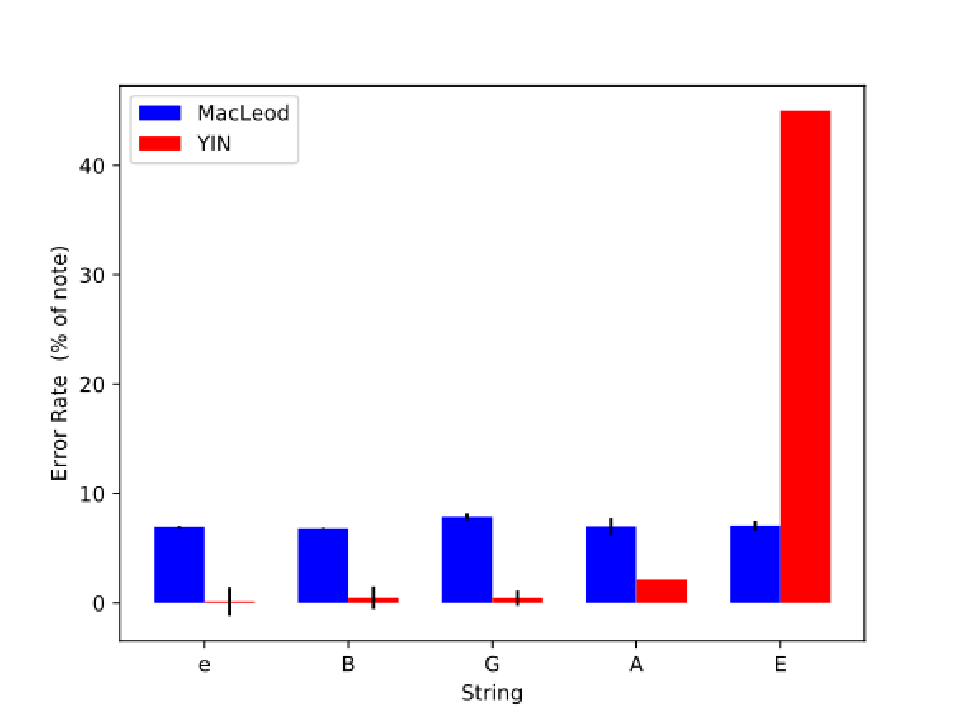
\includegraphics[scale=0.85]{images/measurements/am-chord-error}
  \legend{Source: Authors}
\end{figure}

\begin{figure}[!htpb]
  \centering
  \caption{E chord error}
  \label{e-chord-error}
  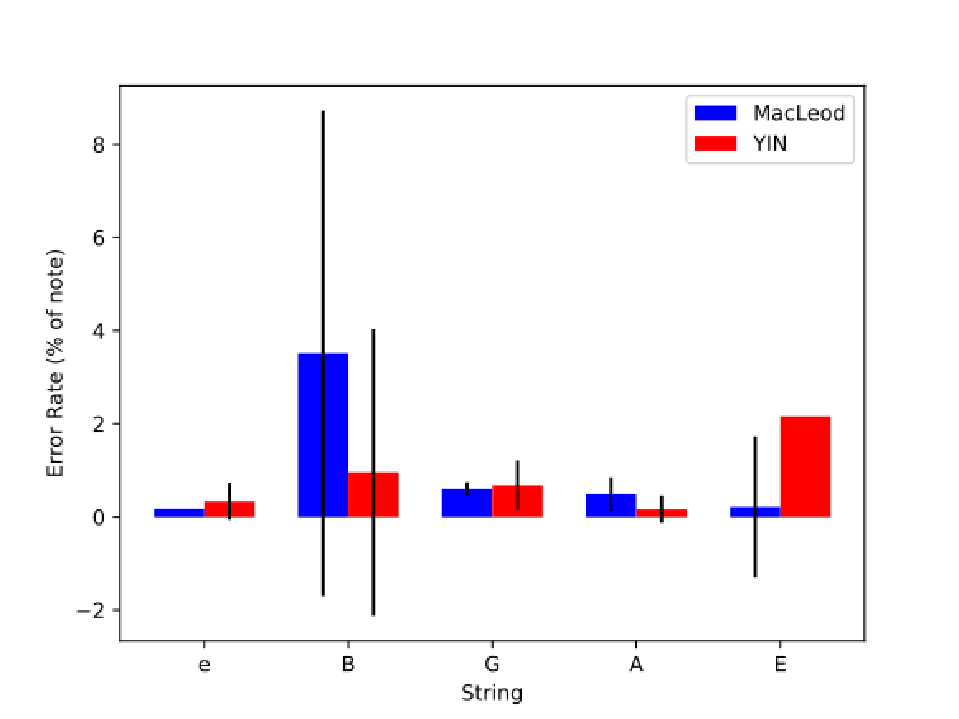
\includegraphics[scale=0.85]{images/measurements/e-chord-error}
  \legend{Source: Authors}
\end{figure}

\section{Chromatic Scale Error}
This experiment aims to assess the performance of the system on detection of notes over time.
Each string is played separately by plucking 5 consecutive
notes (e.g. A, A\#, B, C and C\#) at the speed of approximately 4 notes/s, which can be
considered an usual speed for guitar playing. To avoid pluck miss-detections in this test, repeated
notes are grouped into a single detection. The measurements were then compared with the
expected output, and any miss-detection counted. This test was repeated five times,
and the mean was taken as the error rate, calculated by dividing the number of 
errors by the total number of distinct detected notes. Results in \autoref{chromatic-scale-error}
show that MacLeod presents lower errors in this experiment.

\begin{figure}[!htpb]
  \centering
  \caption{Chromatic scale error}
  \label{chromatic-scale-error}
  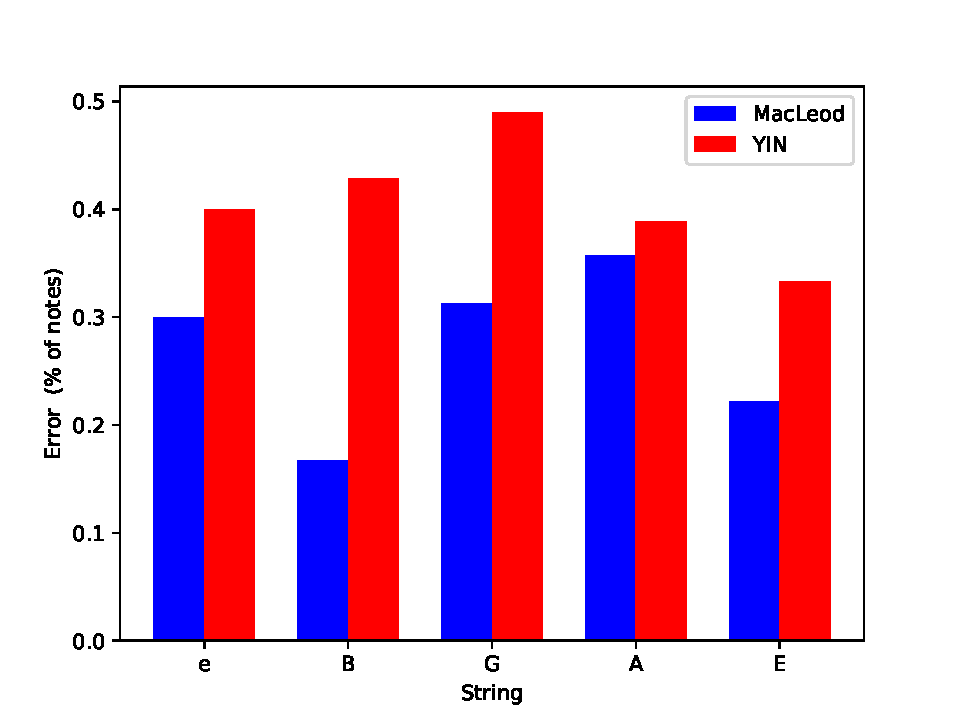
\includegraphics[scale=0.85]{images/measurements/chromatic-scale-error}
  \legend{Source: Authors}
\end{figure}

\section{Pluck Counting} \label{pluck-counting}
In this experiment, several trials of the following procedure are performed for different notes
from the first up to the tenth fret, for all strings: a single note is played 20 times in a row
at a 4 notes/s timing. Thus, the expected global mean of the pluck counting, considering, each
different played note is 20. The obtained values for the MacLeod and YIN were, respectively,
29.9 and 27, corresponding to a 42\% average error. This large error suggests that the simple
amplitude detection by taking the AC mean of the current sampled window is not enough to correctly
detect amplitude changes and more effective methods can be explored, such as \textit{onset detection}.

\section{Discussions}
Strings Single Note Accuracy test provided satisfactory results (\autoref{single-note-accuracy}).
This limited the channel gain which ultimately made this
channel results lower than the others. The same analysis is true for
all other experiments.

Both the chord detection experiments (\autoref{am-chord-error}, \autoref{e-chord-error}) gave reasonable results, but they
show that our system still has lots of room for improvement. The exception is for
the E string error on the Am chord using the YIN algorithm. The reason
for this is that YIN is not working well for low frequency notes, because
it still needs a greater period (samples) for analysis, which is not currently
possible due to processing time limitations - but a solution is proposed at
the next chapter.

The chromatic scale results (\autoref{chromatic-scale-error}) show that our system is not working well along time.
By using a small period of measurement (so it can run at real-time) the range
where a note is changing to the next one is misread as an incorrect result.
This is a big problem for music annotation, but has the same solution as above,
which needs performance improvement.

The last test (\autoref{pluck-counting}) also shows our time related issues,
that, although being natural, still need to be dealt with, for the same reason above, transitions
through time that need a larger sample period to work well, also a better algorithm to detect
amplitude changes. The plucking errors are due to the amplitude detection.
